
\documentclass[final,bibliography=totocnumbered]{include/sikseminar}

\usepackage[utf8]{inputenc} 
\usepackage{todonotes}
\usepackage{hyperref}
\hypersetup{colorlinks = true,linkcolor = black,citecolor = black,urlcolor = black,filecolor = black}
\graphicspath{{./figures/}}
\clubpenalty=10000  
\widowpenalty=10000
%\overfullrule=1mm
\overfullrule=0pt
\begin{document}
%%%%%%%%%%%%%%% TITLEZEUG
\Title[Speicherkonsistenzmodelle für GPUs]{Speicherkonsistenzmodelle für GPUs}
\makeTitle

\Author{Marc Blickle}
\Studiengang{Master Of Science - Informatik}
\makeAuthor

%%%Abgabedatum
\date{14.01.2019}

% Bezeichnung des Seminars
\subject{Safety-Critical Systems }

\maketitle


\begin{abstract}
\section*{Kurzfassung}
Diese Arbeit dreht sich um etablierte Speicherkonsistenzmodelle und inwiefern sie in der Applikationsentwicklung für Grafikchips Anwendung finden können.
Hierzu wird zunächst auf die allgemeine Marktsituation und die Architektur von GPUs eingegangen und warum Shared Memory dabei eine große Rolle spielt.
Nach einem Blick auf bei CPUs Einsatz findende Speicherkonsistenzmodelle wird beschrieben, ob diese den Anforderungen von GPUs an Speicherordnung gerecht werden.
Neuere Architekturen, die eigens für die Verwendung in datenparallelen Systemen entworfen wurden, werden in dieser Arbeit vorgestellt und miteinander verglichen.
\end{abstract}
\thispagestyle{empty}
%%%%%%%%%%%ENDE TITELZEUG

\newpage
%%%%%%%%%%% Inhaltsverzeichnis anzeigen
\tableofcontents

\newpage

%%%%%%%%%%%%%%%%%%%%%%%%%%%%%%%%%%%%%%%%%%%%%%%%%%%%%%%%%%%%%%%%%%%%%%%%%%%%%%%%
% Die eigentliche Arbeit
\newpage
\section{Einleitung}
Prozessoreinheiten mit mehreren Kernen finden schon seit etlichen Jahren Anwendung in Systemen jeder Art: Vom Mobiltelefon, über heimische 
Desktop-PCs bis hin zu mächtigen Serverkonstellationen. Um diesen Prozessoren ein reibungsloses Zusammenspiel mit dem Arbeitsspeicher zu garantieren, ist es von hoher Wichtigkeit, die sich im Verarbeitungsprozess befindlichen Dateien konsistent zu halten. Dies erreicht man mitunter durch
die Entwicklung und Implementation von sogenannten Speicherkonsistenz-Modellen. 
Seit langer Zeit sind CPUs der Prozessortyp, für denen die meisten, nicht grafiklastigen Applikationen entwickelt wurden \cite{syncornot}. Während Graphics Processing Units (GPUs) ursprünglich dazu designed wurden, vor allem Spiele mit ihren grafikbeschleunigenden Eigenschaften zu unterstützen,
hat Ndvidia das Potential  dieser Chips für eine weitsichtigere Anwendung erkannt. Das Unternehmen veröffentlichte daraufhin 2006 die erste GPU, die die CUDA-Architektur unterstützt \cite{cudabe}, 
was das Ausführen von Code ermöglichte, der sich nicht auf grafikbasierte Anwendungen konzentriert.

Mittlerweile bewegt sich der Trend bei der Applikationsentwicklung vermehrt in Richtung paralleler Datenverarbeitung mithilfe von Grafikchips, wie zum Beispiel beim Minen von Bitcoins.
Auch die Hardware, die Jahr für Jahr neu auf den Markt kommt, macht im Gegensatz zum CPU-Segment rasante Fortschritte. 

 Ein großer Mangel stellt hierbei noch das Verwenden geeigneter Speicherkonsistenz-Modelle dar, da das bisherige Anwendungsgebiet von GPUs, nämlich grafisch anspruchsvolle Applikationen, verzeihender bei der Einhaltung der Reihenfolge von Speicheroperationen ist. In den meisten Grafikchips kommen neuartige,  schwache Modelle zum Einsatz, die nur sehr dürftig beschrieben sind.
Dies erschwert es für Entwickler ungemein, neue Applikationen zu verwirklichen.
Der Frage, ob diese schwachen Modelle tatsächlich am sinnvollsten für die Implementierung in einer GPU ist, oder ob es womöglich bessere Alternativen gibt, soll in dieser Seminararbeit auf den Grund gegangen werden.

Dazu werden verschiedene Speicherkonsistenzmodelle, die sich beim Einsatz in CPUs bewährt haben, gegenübergestellt und bezüglich den Anforderungen in GPUs evaluiert. Die Litmustests, die hierzu genutzt werden, sind dazu in der Lage, nützliche Eigenschaften der  Modelle zu beschreiben und sind ein intuitiver Weg diese zu verstehen.
Das am Ende gezogene Fazit fasst die Evaluation zusammen und beschreibt, welches Modell sich am Besten zur Implementierung in Grafikchips eignet.
 
%% NUR CPU ETABLIERTE MODELLE


\newpage
\section{Grundlagen}
\par 
	\subsection{Multicoreprozessoren und Shared-Memory}

Eine Graphics Processing Unit (GPU) ist ein Mikroprozessor, der mit vielen Kernen ausgestattet ist und über eine hohe parallele Datenbandbreite verfügt.
Durch diesen Umstand liegt der Fokus meist eher auf paralleler Performance, als auf Logik und sequentieller Korrektheit in Caches \cite{exploit}.
Er wurde ursprünglich dazu designed, vor allem Spiele mit ihren grafikbeschleunigenden Eigenschaften zu unterstützen, doch seit 2006 werden GPUs auch für gewöhnlichere, datenparallele Rechenaufgaben verwendet, die bis dorthin für CPUs reserviert waren \cite{cudabe}.
Aufgrund der vielen einzelnen Recheneinheiten, die gleichzeitig Aufgaben ausführen, ist es umso wichtiger, Speicherzugriffe zu steuern und zu kontrollieren.
Im Gegensatz zu CPUs verfügt die Speicherarchitektur bei Grafikchips über sehr viele Hierarchieebenen, auch was die Threads angeht  \cite{exploit}.
Diese sind in dreidimensionalen Blöcken (CTA - Coop Thread Array) angeordnet, die wiederum in dreidimensionale Strukturen gruppiert wurden.

Nun teilen sich die sich in den CTAs befindlichen Threads nicht nur einen gemeinsamen Speicher (Shared Memory) pro CTA, sondern auch die CTAs - und somit die sich jeweils darin befindlichen Threads -
greifen auf einen globalen Speicher zu (Global Memory). Shared Memory ist kleiner, dafür schneller als globaler Speicher. Er wird vom GPU-Code selbst deklariert und variiert stark während des Ausführen eines Programmes, 
während globaler Speicher vor der Ausführung vom CPU allokiert und bestimmt wird \cite{gpuhp2}.


\begin{figure}[htbp] %in den eckigen Klammern wird angegeben, wo das Bild erscheinen soll:
					 %h = here, t = top, b = bottom, p = page (eigene Seite für Bild/er)
					 %TeX versucht es in dieser Reihenfolge schön hinzukriegen
					 %wenn das erste gut aussieht, wird das genommen, sonst das zweite usw.
  \centering
% Für die Compilierung mit pdflatex wird z.B. ein .jpg/.png/.pdf Bild
% benötigt. Ein .eps Bild braucht man für die Compilierung mit
% latex. Wird der Dateiname ohne Dateierweiterung (abbildungen/bild)
% angegeben wird je nachdem, ob latex oder pdflatex benutzt wird, die
% entsprechende Datei herausgesucht.
  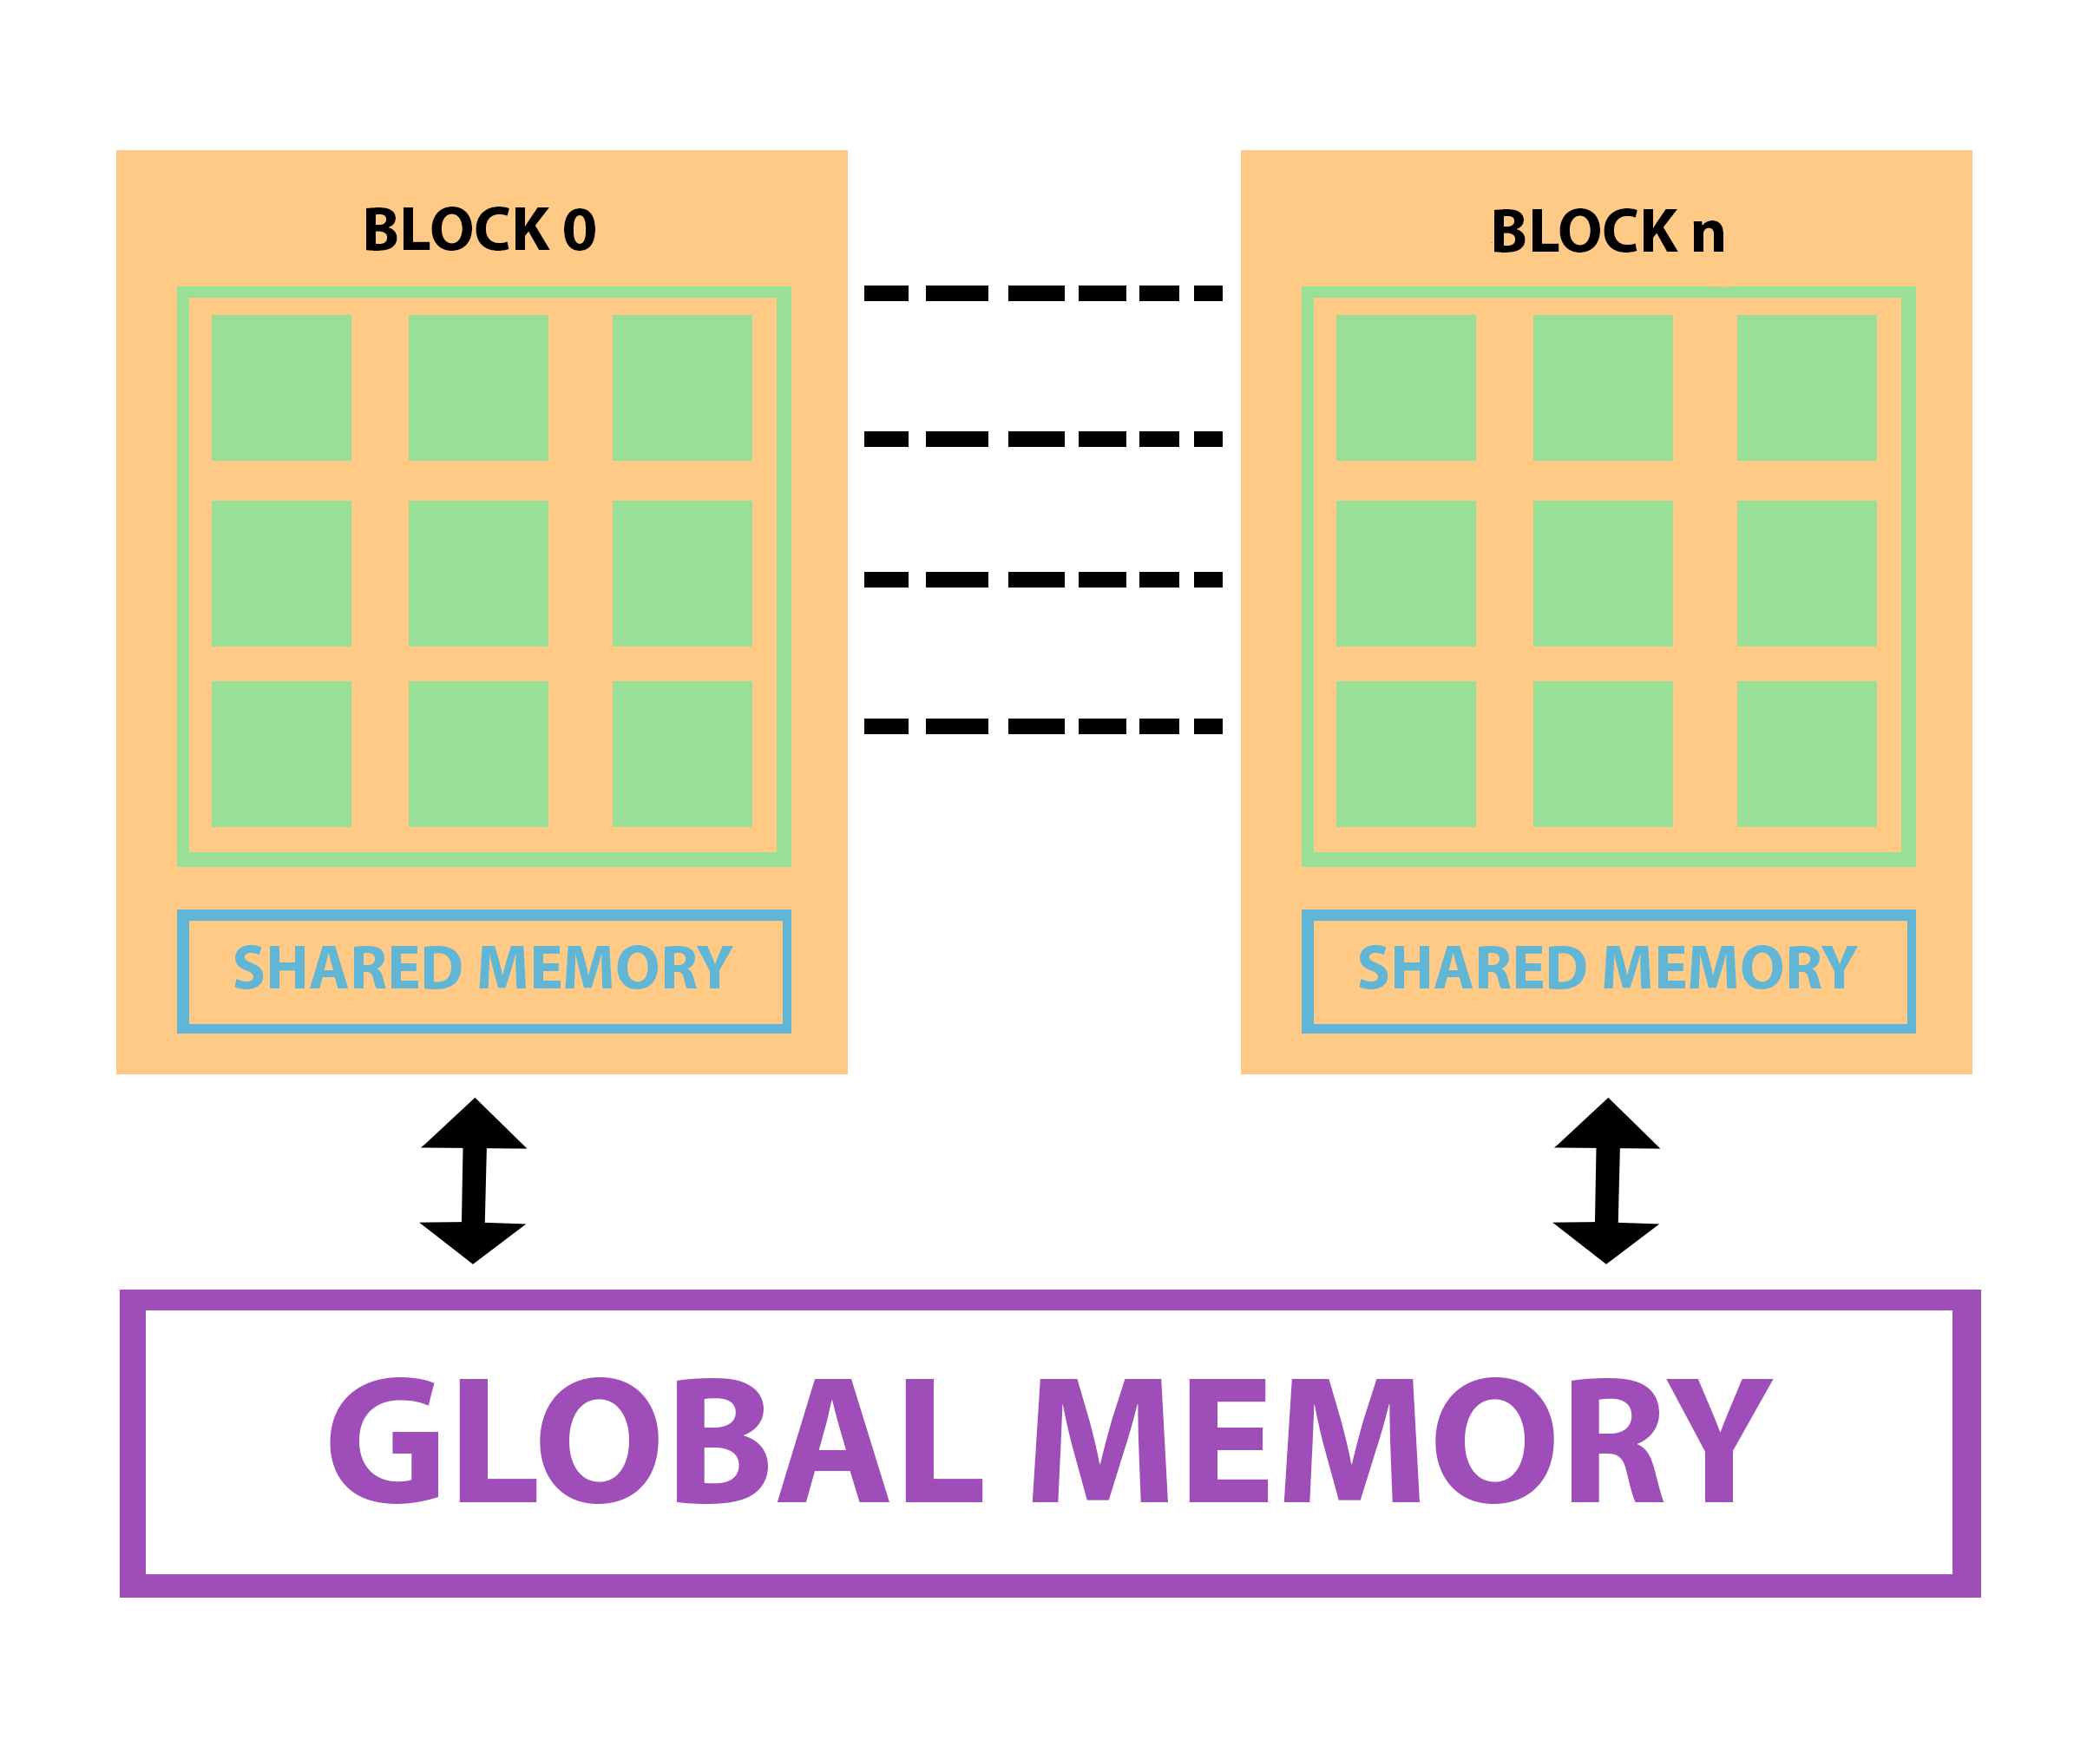
\includegraphics[width=0.5\textwidth]{figures/gpumemory}
  \caption{Verallgemeinerte Ansicht der für diese Arbeit relevanten GPU-Memory-Architektur. Grüne Blöcke stellen Threads dar.}
  \label{Fig:gpum}
\end{figure}


Dieser grundlegenden Struktur lässt sich folgende Phrase ableiten: Auf allen Ebenen muss ein angepasstes Memory-Ordering herrschen.
Grund dafür ist vor allem die schiere Masse an Threads: Der breite Memorybus muss eine große Anzahl davon gleichzeitig versorgen - tausende Reads und Writes 
könnten gleichzeitig den Versuch einer Ausführung starten. Fehlt hierbei die Organisation kann dies eine Verlangsamung (Thread Stalling) oder fehlerhafte Rechenoperationen zur Folge haben, 
woraus eine schlechte Performance resultiert.
Tests haben gezeigt, dass 40-60 Prozent der Performanceeinbußen bei GPUs auf unoptimiertes Speicherhandling zurückzuführen sind \cite{gpuhp2}. %\cite{}.

Man muss also versuchen, stets eine - für die jeweilige GPU-Architektur individuelle - Speicherkonsistenz herbeizuführen.
	
Leider dokumentieren Grafikkartenhersteller die individuelle Architektur ihrer GPUs nur sehr schlecht, was eine optimierte, datenparallele Applikationsentwicklung ungemein erschwert.











	\subsection{Speicherkonsistenz}


Sowohl in der Theorie als auch Praxis tut sich bei Mehrprozessorsystemen zwangsläufig ein schwerwiegendes Problem auf:
Da in solchen Systemen mehrere Prozessoren oder Threads zeitgleich arbeiten, kann und wird es vorkommen, dass mehr als einer gleichzeitig dieselbe Speicheradresse auslesen oder beschreiben möchte.
Dass diese Operationen in der gleichen Reihenfolge ausgeführt werden, in der sie angefordert werden, kann allerdings nicht gewährleistet werden.
Ein simples Beispiel hierfür könnte wie folgt aussehen:
\begin{figure}[htbp] %in den eckigen Klammern wird angegeben, wo das Bild erscheinen soll:
					 %h = here, t = top, b = bottom, p = page (eigene Seite für Bild/er)
					 %TeX versucht es in dieser Reihenfolge schön hinzukriegen
					 %wenn das erste gut aussieht, wird das genommen, sonst das zweite usw.
  \centering
% Für die Compilierung mit pdflatex wird z.B. ein .jpg/.png/.pdf Bild
% benötigt. Ein .eps Bild braucht man für die Compilierung mit
% latex. Wird der Dateiname ohne Dateierweiterung (abbildungen/bild)
% angegeben wird je nachdem, ob latex oder pdflatex benutzt wird, die
% entsprechende Datei herausgesucht.
  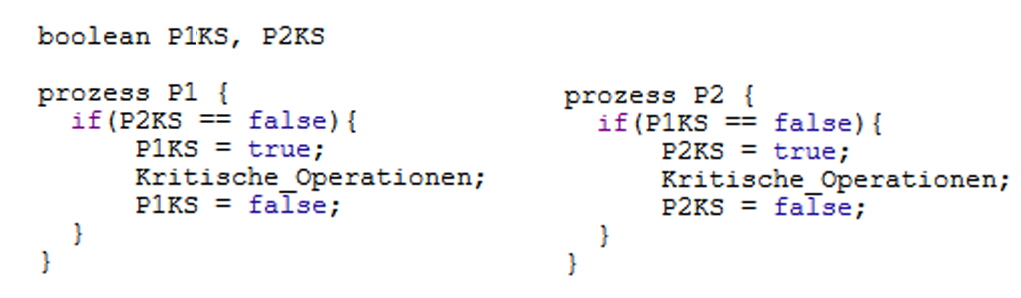
\includegraphics[width=0.7\textwidth]{figures/problem1}
  \caption{Ein simples Problem, bei dem beide Prozesse kritische Operationen ausführen.}
  \label{Fig:problem1}
\end{figure}

Es kann nun vorkommen, dass beide Prozesse zeitgleich die kritischen Operationen ausführen, weil sie nicht wissen dass der jeweils andere Prozess gestartet ist\cite{ocofwmcm}.
Auf dieses Problem sind Dekker und Dijkstra bereits 1965 gestoßen, was zeigt, wie grundlegend solche Schwierigkeiten sind %\cite{CoopSP}.

Dekker war dazu in der Lage, dieses Problem zu lösen, indem er den sogenannten 'Dekker-Algorithmus' entwickelte.
Hierzu änderte er den Code wie in Abbildung 3 dargestellt.
\begin{figure}[htbp] %in den eckigen Klammern wird angegeben, wo das Bild erscheinen soll:
					 %h = here, t = top, b = bottom, p = page (eigene Seite für Bild/er)
					 %TeX versucht es in dieser Reihenfolge schön hinzukriegen
					 %wenn das erste gut aussieht, wird das genommen, sonst das zweite usw.
  \centering
% Für die Compilierung mit pdflatex wird z.B. ein .jpg/.png/.pdf Bild
% benötigt. Ein .eps Bild braucht man für die Compilierung mit
% latex. Wird der Dateiname ohne Dateierweiterung (abbildungen/bild)
% angegeben wird je nachdem, ob latex oder pdflatex benutzt wird, die
% entsprechende Datei herausgesucht.
  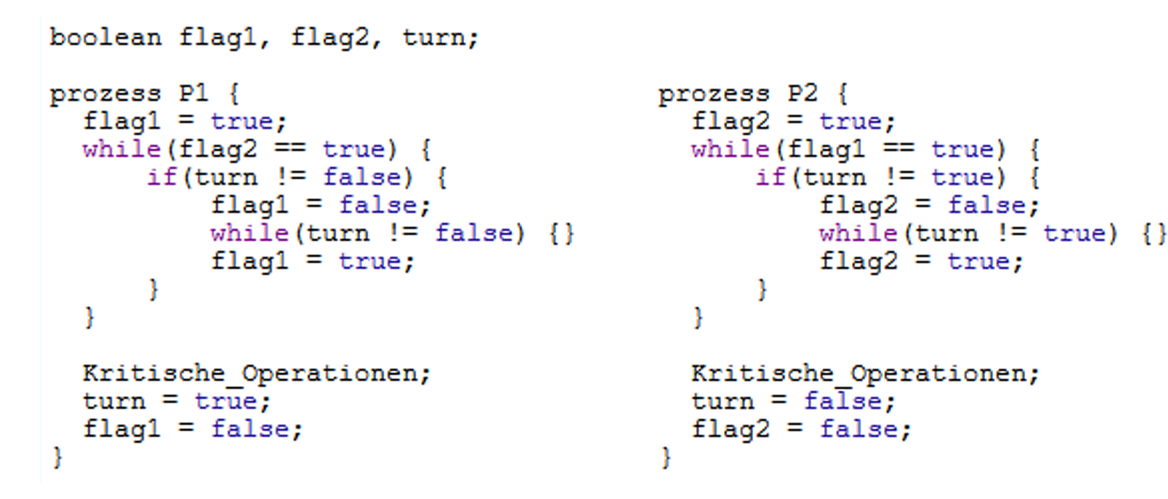
\includegraphics[width=0.7\textwidth]{figures/problem2}
  \caption{Eine Lösung für das in Abbildung 2 gezeigte Problem.}
  \label{Fig:problem2}
\end{figure}

Der Prozess P1 kann nun feststellen, ob P2 beabsichtigt, eine bestimmte kritische Operation auszuführen oder dies sogar schon tut.
Falls beide die Absicht haben, wird mithilfe der Variable 'turn' einem Prozess die Erlaubnis erteilt \cite{ocofwmcm}.

Für Uniprozessor-Systeme ist dies eine fortschrittliche Lösung, falls jedoch keine weiteren Maßnahmen ergriffen werden, scheitert diese Vorgehensweise bei verschiedensten Multiprozessor-Systemen - so zum Beispiel bei solchen, die Operationen in Write-Back Caches speichern.
Beide Prozesse könnten ihre Flagge auf 'true' setzen, doch dieses Write wird im jeweiligen Cache behalten. Somit sehen die Prozesse die jeweilligen Flaggen als 'false' und beide versuchen, kritische Operationen durchzuführen\cite{ocofwmcm}. 


Es zeigt sich also: zu dem Mehrfachzugriff kommt der Umstand, das die zu verwendeten Daten oft mehrfach vorliegen, zum Beispiel in Caches.
Die Zielerreichung einer konsistenten Datenbasis wird folglich ungemein erschwert, da bei jeder Operation jedes Prozessors auf Einheitlichkeit geachtet werden muss.
Nun gibt es zu gegebenem Problem zwei verschiedene Lösungsansätze \cite{ocofwmcm}:
Erstens könnte man das Speichermanagement so lenken, dass es wie bei einem Uniprozessor agiert - man würde eine sequentielle Konsistenz schaffen.
Eine Möglichkeit dies zu tun ist das MESI-Protokoll, welches Cache-Speicherstellen um zwei Statusbits erweitert.
Hierdurch können vier verschiedene Zustände dieser Stellen gespeichert werden, die von anderen Caches gelesen werden können und verhindern,
dass Mehrfachzugriffe entstehen und somit sequentielle Konsistenz schaffen\cite{gpucc}.


Zweitens könnte man schlichtweg akzeptieren, dass man keine sequentielle Konsistenz schaffen kann. Das ist nicht unbedingt schlecht, denn das System kann trotzdem lauffähig sein - vorrausgesetzt, man definiert 
das Speicherverhalten eines Systems und schafft ein Framework für den Programmierer\cite{ocofwmcm}.

Doch was genau ist Konsistenz eigentlich?


\glqq Konsistenz schreibt den Wert vor, den ein Lesezugriff auf eine gemeinsame Variable in einem Multithreadprogramm zurückzugeben vermag\cite{gpucc}.'\grqq

So lautet eine simple Definition für Speicherkonsistenz - doch reicht diese weiter, als zuerst vermutet.
Denn an dieser Stelle kommen die Speicherkonsistenzmodelle ins Spiel,
die beschreiben, wie sich das System im Bezug auf Speicher verhält, wo Grenzen liegen und welche Optimierungen möglich sind \cite{unified}.


Ein solches Modell kann man als Regelwerk betrachten, welches bestimmt, wie das System Speicheroperationen verarbeitet.
Der Programmierer stimmt seine Software so auf diese Regeln ab, damit beim Ausführen von Speicheroperationen die Speicherkonsistenz gewahrt wird.
Die Software, die auf einem solchen System läuft - und somit auch deren Programmierer - müssen sich an die Regeln halten um performantere Ergebnisse zu erzielen.
Jede Code ausführende Komponente ist daran gebunden. Bricht beispielsweise der Compiler eine Regel, so kann auch für die übrigen Komponenten keine korrekte Ausführung mehr garantiert werden.

Es gibt mehrere Facetten, wie solche Regeln und Modelle definiert werden können. Das Offenlegen der Hardwarestruktur, das Definieren von Regeln zur Verwendung von Schnittstellen, das Auferlegen von Programmierrichtlinien oder die direkte Restriktion von Lese- und Schreibzugriffen auf den Speicher sind nur einige der Methoden,
die bei existierenden Modellen angewandt werden \cite{pram}. Sie alle haben aber folgendes gemeinsam:
Je weicher das SKM auf datenparallelen Systemen konstruiert ist, desto komplizierter ist das Programmiermodel, gleichzeitig jedoch steigt die Performance \cite{mcm5,pram}.

Dieser Umstand bedeutet für eine GPU, dass ein möglichst weiches Modell gewählt werden muss. Aus der in Kapitel 2.1 beschriebenen Architektur geht hervor, dass viele tausende Threads gleichzeitig auf den gemeinsamen Speicher zugreifen wollen. Eine sequentielle Anordnung dieser vielen Speicheranfragen würde also einen hohen Aufwand mit sich bringen.
Bei weicheren Modellen können sich Anfragen unter Umständen jedoch auch überschneiden oder bieten ähnliche Mechanismen, die eine schnellere Ausführung der Operationen garantieren. Datenparallele Multiprozessoren sind diesbezüglich also vor allem auf Performance ausgelegt, die durch leichte Modelle leichter erzielt werden kann. 

%CITE LIpton SANdberg 88
%cite adve 93

%Choosing a Model is atradeoff between minimizing memory access order constraints and the comlexity of the protgramming model, as well as of the complexity of the memory model itslf
%In general, the programming model becomes more restricted and complicated as the consistency model becomes weaker.
%Weaker Memory Consistency Models can have a positive effect on the performance of parallel shared memory machines, the benefit increases as memory latency increases









\section{Speicherkonsistenzmodelle}
In den folgenden Kapiteln werden die Modelle unter anderem mithilfe von litmus-Tests beschrieben.
Sie zeigen oftmals die Besonderheiten eines SKMs auf und vermitteln dessen Eigenschaften auf einer anwendungsbasierten Ebene.

	\subsection{Klassische Speicherkonsistenzmodelle}
	\subsubsection{Sequential Consistency Model}

Die sequentielle Konsistenz wurde erstmals von Lamport im Jahre 1979 wie folgt beschrieben \cite{lamp}: 

\glqq The result of any execution is the same as if the operations of all the processors were executed in some sequential order, and the operations of each individual processor appear in this sequence in the order specified by its program.\grqq
Das bedeutet, dass um Konsistenz zu erzielen

- Jeder Prozessor Speicheranfragen in der Reihenfolge einreicht, die ihm vom Programm vorgegeben wurden

- Speicheranfragen jedes einzelnen Prozessors von einer einzigen Queue verarbeitet werden, die die einzelnen Anfragen sortiert

Im Wesentlichen wird eine festgelegte Reihenfolge für verschiedene, gleichzeitige Operationen gewählt. Diese Reihenfolge ist global und muss von allen Prozessoren beachtet werden \cite{smcmtutorial,unified}.

\begin{figure}[htbp] %in den eckigen Klammern wird angegeben, wo das Bild erscheinen soll:
					 %h = here, t = top, b = bottom, p = page (eigene Seite für Bild/er)
					 %TeX versucht es in dieser Reihenfolge schön hinzukriegen
					 %wenn das erste gut aussieht, wird das genommen, sonst das zweite usw.
  \centering
% Für die Compilierung mit pdflatex wird z.B. ein .jpg/.png/.pdf Bild
% benötigt. Ein .eps Bild braucht man für die Compilierung mit
% latex. Wird der Dateiname ohne Dateierweiterung (abbildungen/bild)
% angegeben wird je nachdem, ob latex oder pdflatex benutzt wird, die
% entsprechende Datei herausgesucht.
  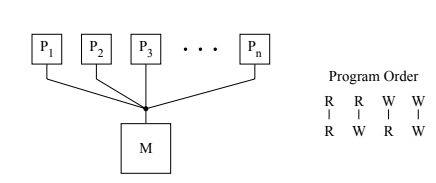
\includegraphics[width=0.7\textwidth]{figures/seqq}
  \caption{Veranschaulichung der Programorder, unter der die sequentielle Konsistenz gültig ist\cite{mcm3}.}
  \label{Fig:seqq}
\end{figure}
Grafik 4 zeigt, dass sich die einzelnen Prozessoren in einer Schlange befinden, die nach und nach auf den Arbeitsspeicher zugreifen dürfen.
In der auf der rechten Seite dargestellten Programordner wird deutlich, dass eine Leseoperation (R) warten muss, bis die vorangegangene Leseoperation abgeschlossen wurde. Indikator hierfür ist der einfache, durchgezogene Strich zwischen den Buchstaben.
'W' steht hierbei für eine Schreiboperation\cite{designingmcm}: 'W' muss auf 'R' warten, 'R' auf 'W' und 'W' wartet ebenso auf vorangegangene Schreiboperationen.  

In einer abstrahierten Betrachtung sind alle Prozessorunits über einen Switch an den globalen Speicher gekoppelt. Die Aufgabe des Switches ist es nun, den Speicher für einen Prozessor freizugeben, der daraufhin Operationen ausführen darf.
Er gibt nach und nach weitere Prozessoren frei, die schließlich an den Switch zurückmelden, sodass dieser die Operationen fein säuberlich sortieren kann, was zu einer sequentiellen Ordnung führt. 
Daraus folgt auch, dass jeder Prozessor immer genau dieselbe Reihenfolge an Operationen sieht wie alle anderen Prozessoren, egal in welcher Reihenfolge sie eingereicht wurden \cite{smcmtutorial}.

Wie im folgenden Bild 5 zu sehen, soll von Prozessor 3 ein Wert erfasst werden, der noch gar nicht existiert. Dies symbolisiert eine gewisse Flexibilität, auch wenn dies in einem realen System nicht angewandt werden könnte. Die Operation R(y)2 versucht hier einen Wert zu lesen, der noch gar nicht geschrieben wurde. Die Flexibilität wird insofern umgesetzt, dass 
das System diese Operation zeitlich nach der Writeoperation(y) setzen würde.

\begin{figure}[htbp] %in den eckigen Klammern wird angegeben, wo das Bild erscheinen soll:
					 %h = here, t = top, b = bottom, p = page (eigene Seite für Bild/er)
					 %TeX versucht es in dieser Reihenfolge schön hinzukriegen
					 %wenn das erste gut aussieht, wird das genommen, sonst das zweite usw.
  \centering
% Für die Compilierung mit pdflatex wird z.B. ein .jpg/.png/.pdf Bild
% benötigt. Ein .eps Bild braucht man für die Compilierung mit
% latex. Wird der Dateiname ohne Dateierweiterung (abbildungen/bild)
% angegeben wird je nachdem, ob latex oder pdflatex benutzt wird, die
% entsprechende Datei herausgesucht.
  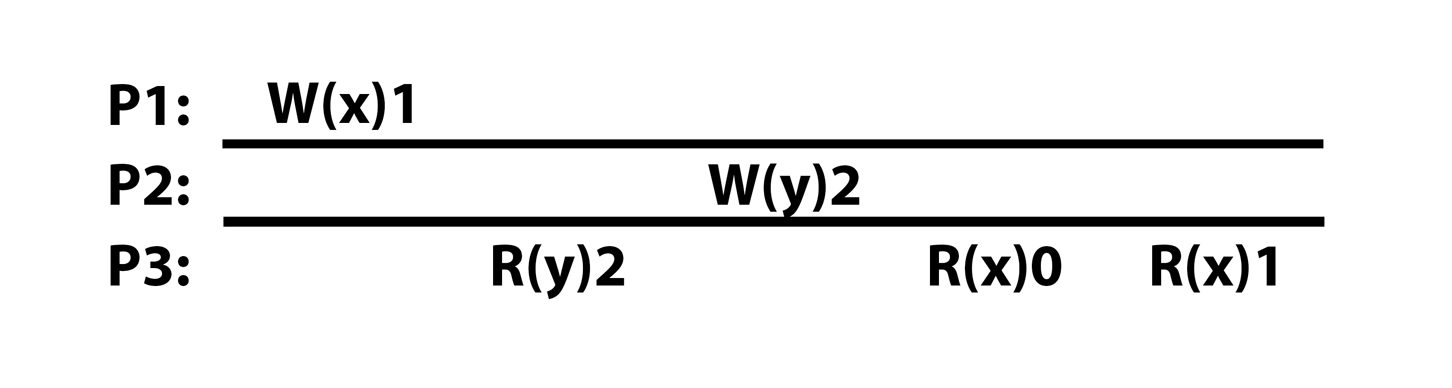
\includegraphics[width=0.7\textwidth]{figures/SeqModell1}
  \caption{So koennte ein Ablauf unter Verwendung des sequentiellen Modells aussehen. Die einzelnen Operationen überschneiden sich niemals \cite{mcm5}.}
  \label{Fig:SeqModell1}
\end{figure}

Die folgende Grafik 6 zeigt eine einfachere Darstellung eines Programms. Unter sequentiell konsistenten Aspekten ist es unmöglich, 
dass das Tupel (y,x)=(2,1) geprintet wird. Möglich wäre jedoch (2,3),(4,3) und (4,1).
\begin{figure}[htbp] %in den eckigen Klammern wird angegeben, wo das Bild erscheinen soll:
					 %h = here, t = top, b = bottom, p = page (eigene Seite für Bild/er)
					 %TeX versucht es in dieser Reihenfolge schön hinzukriegen
					 %wenn das erste gut aussieht, wird das genommen, sonst das zweite usw.
  \centering
% Für die Compilierung mit pdflatex wird z.B. ein .jpg/.png/.pdf Bild
% benötigt. Ein .eps Bild braucht man für die Compilierung mit
% latex. Wird der Dateiname ohne Dateierweiterung (abbildungen/bild)
% angegeben wird je nachdem, ob latex oder pdflatex benutzt wird, die
% entsprechende Datei herausgesucht.
  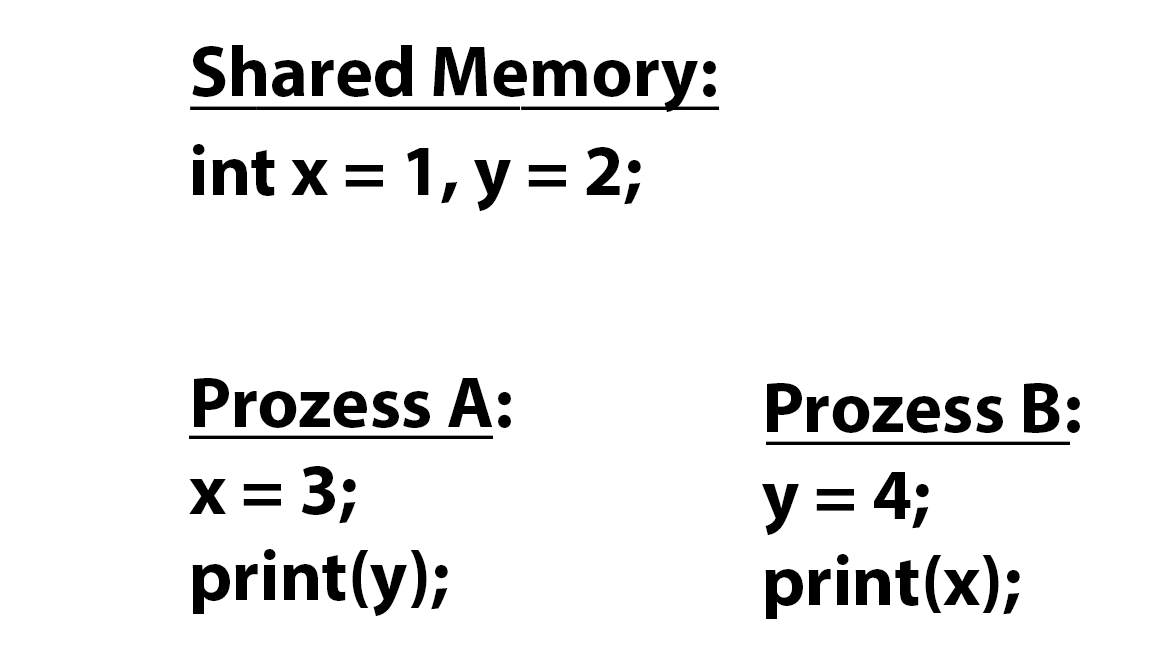
\includegraphics[width=0.7\textwidth]{figures/sc2}
  \caption{Ein weiteres Beispiel von SC, an den Dekker's Algorithmus angelehnt.}
  \label{Fig:sc2}
\end{figure}

Die Programorder impliziert, dass auf x=3 print(y) folgt und auf y=4 print(x) folgt.
Als nächstes nimmt man an, dass print(y) eine 2 ausspuckt. Deshalb kann davon ausgegangen werden,
dass auf print(y) y =4 folgt, weil sonst bei print(y) eine andere Ausgabe erfolgt wäre. Also kann man schließen, dass print(x) nach x = 3 stehen muss.
X = 3 -> print(x) besagt, dass x=3 sein muss. Nach der gleichen Logik ist y=2. Man erhält also das Tupel (2,3). 

Gleichermaßen lässt sich der Prozess B an erste Stelle stellen, jedoch kommt man nie zu einem Tupel (2,1), was zu einer sequentiellen Konsistenz führt.

Bei genauerem Hinsehen fällt auf, dass dessen Abläufe stark der Denkweise eines Software-Entwicklers ähneln \cite{eesmog}
, deshalb
war dieses Modell lange Zeit Go-To-Variante, noch heute ist es allgegenwärtig. Das Problem hierbei ist, dass die Idee eines sequentiell konsistenten Modells nicht wirklich zu einem Multiprozessorsystem passt und die Speicherleistung hemmt \cite{msssm}.
  Allerdings wird sich zwischenzeitlich im Multicore-Bereich eher auf schwächere Alternativen konzentriert, da diese mehr Raum für Verbesserungen und Leistungssteigerung zulassen.



Das System gilt als konsistent, wenn unter allen Operationen jedes Prozessors eine Programmordnung eingehalten wird, als wäre es ein Prozessor.
Dieser Umstand ist nicht gut für GPUs, weil es hier sehr viele Threads gibt, die alle beachtet werden müssen: Jedes Mal, wenn ein Prozessor eine Speicheroperation ausführt, müssen alle anderen Prozessoren, die dies auch wollen, auf die Fertigstellung der ersten Operation warten.


	\bigskip



	\subsubsection{Weak Consistency Model}


Zuerst von Dubois 1986 vorgestellt,
wurden schwache Speichermodelle extra zu dem Zweck entwickelt, die Speicherlatenz - also die Zeit zwischen Anfrage und Erhalt eines Wertes vom Prozessor - zu verringern \cite{mcm3}.
Sie entstanden aus der Weiterentwicklung des sequentiellen Models heraus: Es wurde so abgeschwächt, dass für das sequentielle Modell inkonsistente Status ermöglicht wurden.
Anhand von Simulationen konnte nachvollzogen werden, das dies zu einer Leistungssteigerung von bis zu 40 Prozent gegenüber rein sequentiellen Modellen führen kann\cite{mcm5}.

Sämtliche Ordnung wird aufgegeben, man hat zunächst keinen Überblick darüber, in welcher Reihenfolge Operationen ausgeführt werden.
Das hat zur Folge, dass der Programmierer beim Entwickeln oder Anpassen seiner Software vorsichtig sein muss und die Operationen genau synchronisieren muss, sobald die Ausführungsreihenfolge 
ein kritischer Faktor ist \cite{designingmcm}.

Aus diesem neuen Konzept entstanden die 'Weak Consistency Models' (WCM), die ein sehr striktes Regelwerk mit sich bringen.
 


Schwache Konsistenz gilt als erfüllt \cite{mcm5}\cite{mcm}\cite{unified}, wenn

- alle Variablen, die mit Synchronisationsoperationen zu tun haben, stets von allen Prozessoren in derselben sequentiellen Reihenfolge gesehen werden können 

- alle anderen Operationen in beliebiger Reihenfolge von unterschiedlichen Prozessoren gesehen werden können

- alle Synchronisationsoperationen abgeschlossen sind bevor eine Datenoperationen stattfinden kann und umgekehrt

- die Gesamtheit von Read- und Writeoperationen zwischen verschiedenen Synchronisationsoperationen dieselbe in jedem Prozess ist, also die Synchronisationsoperationen sequentiell konsistent sind



Realisiert werden diese Regeln und Bedingungen wie folgt:

Jede Recheneinheit ist dazu in der Lage, zwei verschiedene Arten von Operationen auszuführen. Auf der einen Seite sind das 
gewöhnliche Datenoperationen, bei denen Werte aus dem Speicher gelesen und geschrieben werden. 
Doch da es keine einheitliche Sichtbarkeit von Speicheroperationen gibt, können andere Prozessoren nicht immer die bereits errechneten, neuen Werte sehen \cite{mcm5}. 
Deshalb ist jede Einheit zusätzlich dazu in der Lage, eine weitere Operation auszuführen: eine Synchronisation. Eine Synchronisation kann als Neuanordnung der Speicheroperationen gesehen werden. Hierbei wird versucht, eine optimale Reihenfolge zu generieren um die Performance zu steigern.
Wenn diese von einem Prozessor getriggert wird, dürfen keine neuen Daten- oder Synchronisationsoperationen begonnen und alle Writes müssen zum Abschluss gebracht werden.
Dies wird dadurch erreicht, dass jeder Prozessor einen Counter über seine noch offenen Operationen führt. Erst wenn alle Counter auf Null stehen, dürfen wieder neue Rechenanfragen und Synchronisationen gestartet werden.
Dieser Zustand hält solange an, bis die Synchronisation durchgeführt ist. Um eine Ordnung zwischen mehreren Operationen zu schaffen muss also mindestens eine Synchronisation ausgeführt werden.

Abbildung 7 schlüsselt den Programmablauf weiter auf:
\begin{figure}[htbp] %in den eckigen Klammern wird angegeben, wo das Bild erscheinen soll:
					 %h = here, t = top, b = bottom, p = page (eigene Seite für Bild/er)
					 %TeX versucht es in dieser Reihenfolge schön hinzukriegen
					 %wenn das erste gut aussieht, wird das genommen, sonst das zweite usw.
  \centering
% Für die Compilierung mit pdflatex wird z.B. ein .jpg/.png/.pdf Bild
% benötigt. Ein .eps Bild braucht man für die Compilierung mit
% latex. Wird der Dateiname ohne Dateierweiterung (abbildungen/bild)
% angegeben wird je nachdem, ob latex oder pdflatex benutzt wird, die
% entsprechende Datei herausgesucht.
  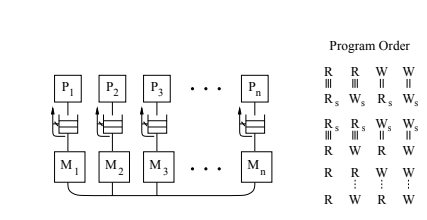
\includegraphics[width=0.9\textwidth]{figures/weeeea}
  \caption{Programmablauf bei dem Weak Consistency Model \cite{mcm3}.}
  \label{Fig:weak}
\end{figure}


 'Rs' und 'Ws' deklarieren Operationen, die als Synchronisation ausgewiesen sind. 'R' und 'W' stellen hierbei Read- und Writeoperations dar, diese können auch als Synchronisation fungieren.
Die doppelten Linien zwischen Operationen indizieren, dass es Unteroperationen geben kann, die alle fertiggestellt werden müssen,
bevor dies mit der übergeordneten geschehen kann: So gesehen bei sämtlichen Writeoperationen, denen eine Synchronisation folgt und bei sämtlichen 
Synchronisationswrites, denen eine beliebige Operation nachfolgend ist, wie zuvor bereits beschrieben.
Drei Linien stehen dafür, dass die nachfolgende Readoperationen ihren Wert zurückliefern muss, bevor weitere Operationen derselben vorangegangenen Operation folgen dürfen \cite{mcm3}.
Der Unterschied zum sequentiellen Modell, der vor allem ins Auge fällt, ist dass Lese- nicht auf Leseoperationen warten müssen. Ebenso muss eine Schreiboperation nicht auf eine Leseoperation warten, außer beide möchten auf dieselbe Speicheradresse zugreifen.
Indikator hierfür ist die gestrichelte Linie. Auch die übrigen in der Grafik aufgeführten Regeln verdeutlichen, dass es mehr Flexibilität bei dieser Programorder gibt, weil weniger sequentiell gehalten werden muss.

Angenommen, es stünde eine kritische Writeoperation an. Wenn diese nun mehrere Speicherzugriffe benötigen würde, so müsste bei einem sequentiellen Modell jeder Write auf den jeweils Vorangehenden warten. Hält sich der Programmierer an die Vorgaben des Weak Consistency Models sorgt er jedoch dafür, dass kein anderer Prozess Zugriff auf diese kritischen Daten haben muss, bevor sie nicht komplett geschrieben wurden, was das Warten überflüssig macht \cite{mcm}. 
\begin{figure}[htbp] %in den eckigen Klammern wird angegeben, wo das Bild erscheinen soll:
					 %h = here, t = top, b = bottom, p = page (eigene Seite für Bild/er)
					 %TeX versucht es in dieser Reihenfolge schön hinzukriegen
					 %wenn das erste gut aussieht, wird das genommen, sonst das zweite usw.
  \centering
% Für die Compilierung mit pdflatex wird z.B. ein .jpg/.png/.pdf Bild
% benötigt. Ein .eps Bild braucht man für die Compilierung mit
% latex. Wird der Dateiname ohne Dateierweiterung (abbildungen/bild)
% angegeben wird je nachdem, ob latex oder pdflatex benutzt wird, die
% entsprechende Datei herausgesucht.
  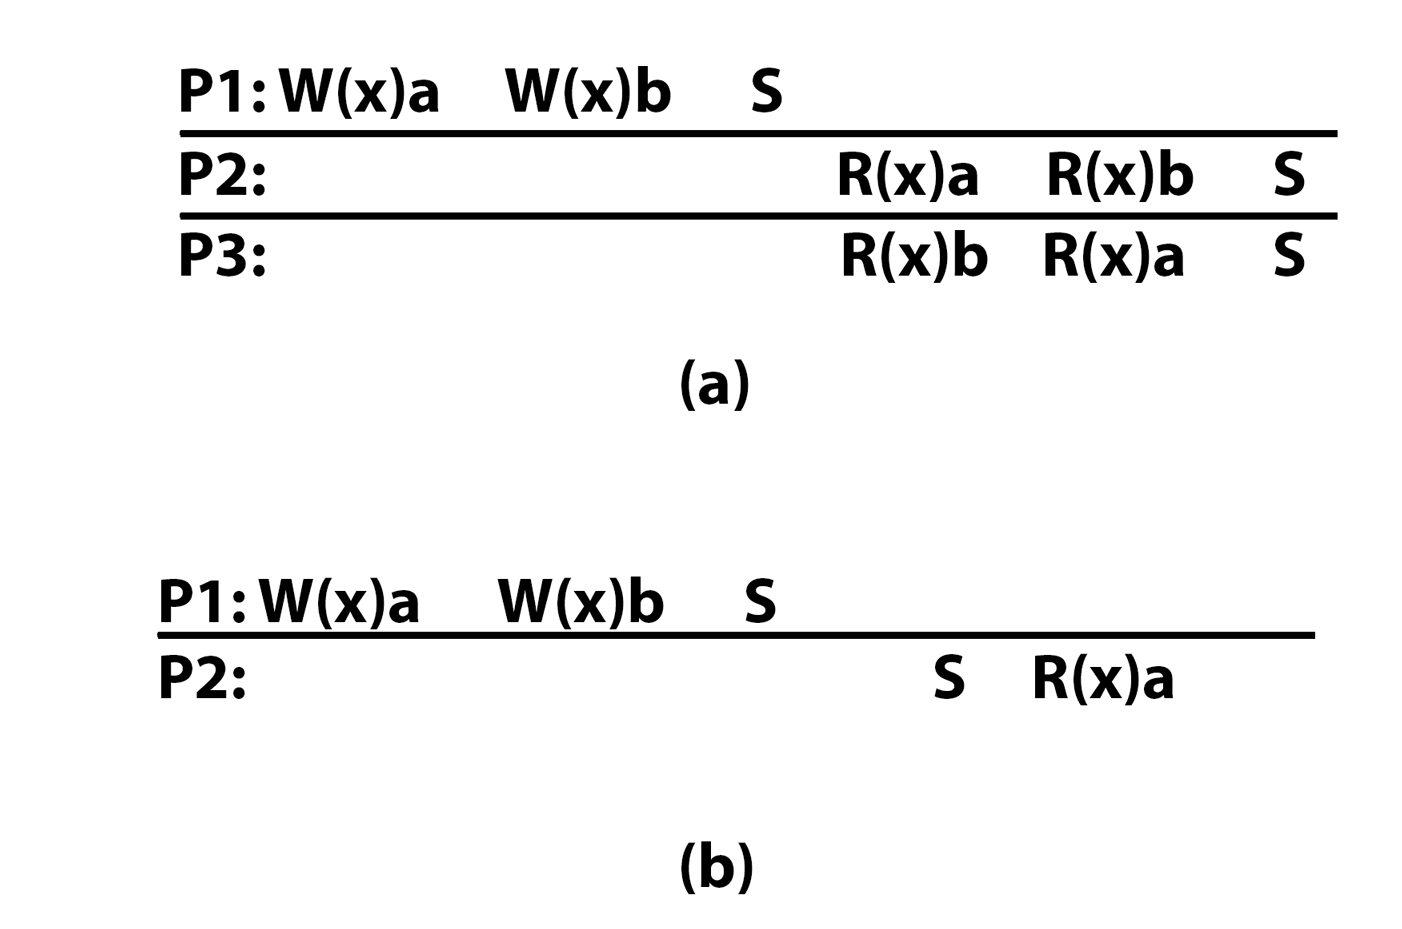
\includegraphics[width=0.9\textwidth]{figures/weaklit}
  \caption{Ein Test, der aufzeigt, wie die Operationen aneinander gereiht werden. \cite{}}
  \label{Fig:weak}
\end{figure}

Abbildung 8 zeigt ein Beispiel für einen Programmablauf unter Einhaltung der weichen Konsistenz, die durch die Synchronisationsoperationen ('S') sichergestellt werden kann.

Der Vorteil, der sich also bei dieser Art von Modell für eine GPU ergibt ist, dass sich die einzelnen Threads in beliebiger Reihenfolge Zugriff verschaffen können und somit nicht auf andere Prozesse warten müssen: 
das verringert die Latenz  und somit eine Performancesteigerung, die laut Tests bei bis zu 60 Prozent liegen kann \cite{exploit}. 

Hierbei könnte es  vorkommen, dass Speicher verwendet werden will, der schon in Benutzung ist und somit ein inkonsistenter Status herbeigerufen wird. Aber eben diesen Umstand kann der Programmierer mithilfe 
von sinnvoll eingesetzten Synchronisationsoperationen verhindern. Vor allem bei kritischen Operationen, bei denen es auf die Reihenfolge ankommt,
durchgeführt werden.
Ein Fehler, der hierbei gemacht werden kann, ist die übermäßige Synchronisation, die auch Ressourcen verbraucht. Wird diese zu oft ausgeführt, wird der gewonnene Performancevorteil wieder zunichte gemacht. Außerdem muss der Programmierer von vornherein alle Synchronisationszugriffe deklarieren, was einen höheren Arbeitsaufwand mit sich bringt.
Heutzutage sind sie sehr stark in datenparallelen Shared-Memory Systemen vertreten.





%\cite{ATUTORIAOL}
	\subsubsection{Release Consistency Model}

Das Release Consistency Model ist eine Weiterentwicklung der schwachen Konsistenz. Der Hauptunterschied ist hierbei die weitere Unterteilung der Synchronisationsoperationen in 'aquire' und 'release' \cite{smcmtutorial}.

'Aquire' funktioniert wie die Synchronisation bei WCM, jedoch überprüft es nur, ob alle Schreiboperationen auf den gemeinsamen Daten beendet sind. Erst wenn dies der Fall ist, erhält der ausführende Prozessor exklusiven Zugriff. Es ist also eine Funktion zum Anfragen von Berechtigungen und gilt als Leseoperation.
'Release' funktioniert auch wie die Synchronisation bei WCM, allerdings in die andere Richtung wie 'aquire': Mit dieser Funktion kann der Prozessor alle Schreiboperationen frei zugänglich machen, muss allerdings selbst noch nicht mit schreiben fertig sein \cite{mcm,designingmcm}. Dies ist also eine Funktion zum gewähren von Berechtigungen und gilt als Schreiboperation.
Möchte ein anderer Prozessor trotzdem zugreifen, kann er 'aquire' verwenden. 



\begin{figure}[htbp] %in den eckigen Klammern wird angegeben, wo das Bild erscheinen soll:
					 %h = here, t = top, b = bottom, p = page (eigene Seite für Bild/er)
					 %TeX versucht es in dieser Reihenfolge schön hinzukriegen
					 %wenn das erste gut aussieht, wird das genommen, sonst das zweite usw.
  \centering
% Für die Compilierung mit pdflatex wird z.B. ein .jpg/.png/.pdf Bild
% benötigt. Ein .eps Bild braucht man für die Compilierung mit
% latex. Wird der Dateiname ohne Dateierweiterung (abbildungen/bild)
% angegeben wird je nachdem, ob latex oder pdflatex benutzt wird, die
% entsprechende Datei herausgesucht.
  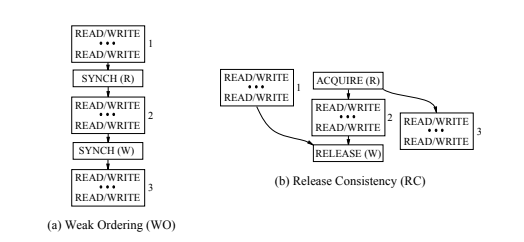
\includegraphics[width=0.8\textwidth]{figures/compare}
  \caption{RC und WC im Vergleich\cite{mcm3}.}
  \label{Fig:compare}
\end{figure}

%%%%BILD COMPARE

Eine Release Consistency oder Freigabekonsistenz ist sichergestellt \cite{designingmcm}, wenn

- alle Schreiboperationen einer Unit A werden von einer anderen Unit B gesehen, nachdem Unit A sie released hat und bevor Unit B sie aquired hat

- alle 'aquire'-Operationen durchlaufen sind, bevor geschrieben oder gelesen wird

- alle Schreib- oder Leseoperationen durchlaufen sind, bevor ein 'release' startet

Verdeutlichen soll dies die folgende Programmordnung.

%%%%BILD RC
\begin{figure}[htbp] %in den eckigen Klammern wird angegeben, wo das Bild erscheinen soll:
					 %h = here, t = top, b = bottom, p = page (eigene Seite für Bild/er)
					 %TeX versucht es in dieser Reihenfolge schön hinzukriegen
					 %wenn das erste gut aussieht, wird das genommen, sonst das zweite usw.
  \centering
% Für die Compilierung mit pdflatex wird z.B. ein .jpg/.png/.pdf Bild
% benötigt. Ein .eps Bild braucht man für die Compilierung mit
% latex. Wird der Dateiname ohne Dateierweiterung (abbildungen/bild)
% angegeben wird je nachdem, ob latex oder pdflatex benutzt wird, die
% entsprechende Datei herausgesucht.
  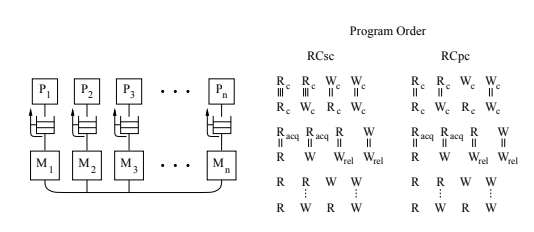
\includegraphics[width=0.8\textwidth]{figures/rc}
  \caption{Programorder bei RC\cite{mcm3}.}
  \label{Fig:rc}
\end{figure}

Release Consistency wird, wie in Abbildung 10 gezeigt, %%%BILD
in zwei Arten unterteilt. Sie unterscheiden sich lediglich in der Reihenfolge, in der Synchronisationsoperationen ausgeführt werden dürfen.

Bei RCsc wird Sequential Consistency unter allen Syncs bewahrt, während bei RCpc processor consistency(PC) bewahrt wird \cite{mcm3}.
PC bedeutet, dass die Reihenfolge, in der Prozessoren die Schreiboperatioen jedes beliebigen Prozessor sehen, dieselbe ist in der die Operationen erteilt wurden \cite{smcmtutorial}.
Die zwei Arten unterscheiden sich abgesehen vom Programmablauf jedoch in keinster Weise. 
Der Unterschied zu WC ist hierbei, dass eine Leseoperation den Wert einer Schreiboperation, der sich allerdings noch im Buffer befindet, zurückgeben darf \cite{smcmtutorial}.

\begin{figure}[htbp] %in den eckigen Klammern wird angegeben, wo das Bild erscheinen soll:
					 %h = here, t = top, b = bottom, p = page (eigene Seite für Bild/er)
					 %TeX versucht es in dieser Reihenfolge schön hinzukriegen
					 %wenn das erste gut aussieht, wird das genommen, sonst das zweite usw.
  \centering
% Für die Compilierung mit pdflatex wird z.B. ein .jpg/.png/.pdf Bild
% benötigt. Ein .eps Bild braucht man für die Compilierung mit
% latex. Wird der Dateiname ohne Dateierweiterung (abbildungen/bild)
% angegeben wird je nachdem, ob latex oder pdflatex benutzt wird, die
% entsprechende Datei herausgesucht.
  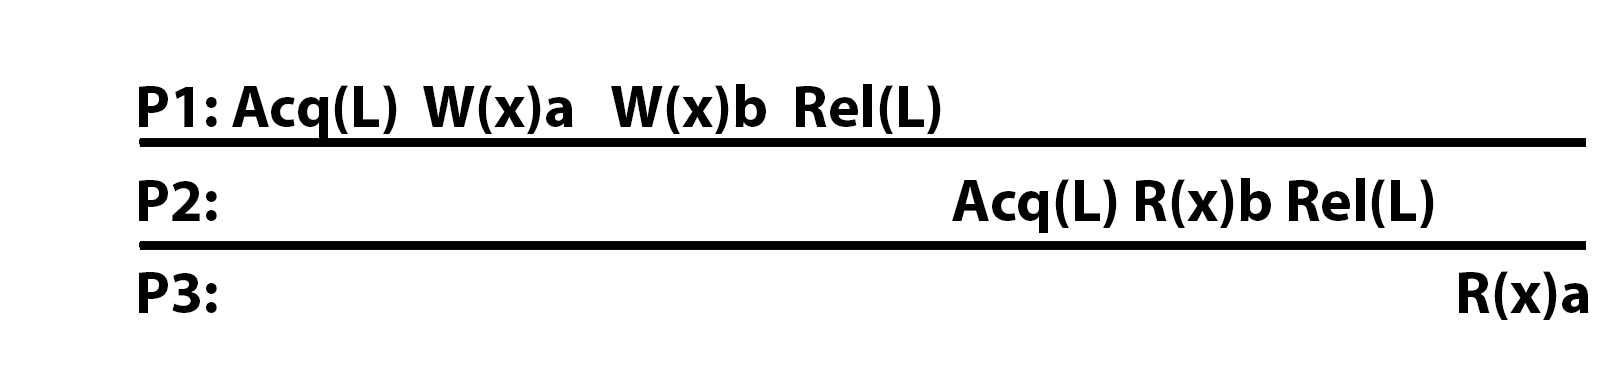
\includegraphics[width=0.8\textwidth]{figures/rellit}
  \caption{Programmbeispiel unter Einhaltung von Release Consistency. \cite{}}
  \label{Fig:rc}
\end{figure}

Abbildung 11 zeigt einen Programmablauf unter Einhaltung der Release Consistency. Sie verdeutlicht, wie die einzelnen 'release'- und 'aquire'-Operationen abgesetzt werden müssen. Wie in Abbildung 10 beschrieben, muss hierbei der Prozessor 3 keinen 'acquire'-Befehl absetzen.

Der wichtigste Veränderung bei RC ist also folgende: 'release' muss auf vorangegangene Operationen warten, folgende Operationen warten aber nicht auf die Fertigstellung von 'release'. Ebenso muss 'aquire' nicht auf vorangegangene Operationen warten, weil es keine Rechte für das Lesen oder Beschreiben vorangegangener Speicheroperationen vergeben muss.
Das Ergebnis sind mehr Flexibilität und Schnelligkeit zwischen 'acquire' und 'release'.
Verdeutlicht wird dies in Abbildung 9: %%% 
RC verfügt im Gegensatz zu WC über die Fähigkeit, Operationen überlappen zu lassen.
Zwar wird dadurch mehr Rechenleistung benötigt, jedoch erreicht man durch die Zeitersparnis eine zusätzliche Performancesteigerung zu sequentiellen Modellen.








	\subsection{Herangehensweise für GPUs}

Sollen im vorherigen Kapitel vorgestellte und andere Speicherkonsistenzmodelle für GPUs implementiert werden,
reicht es nicht aus, die bereits für CPUs bestehenden Frameworks anzuwenden, weil diese über eine viel flachere Speicherhierarchie verfügen \cite{gpucc}.
Zumindest werden sie als flach dargestellt, da die von Caches herbeigeführte Hierarchie oft nicht vom Programmierer miteinzubeziehen ist.
Bei GPUs ist dies nicht nur möglich, sondern notwendig. Weil sowohl Threads als auch Speicher auf einer stark hiararchischen Ebene fungieren - wie im Grundlagenkapitel beschrieben -%%%%%
muss auch hierarchisch gemanaged werden.

Im Folgenden werden deshalb zwei Ansätze beschrieben, dieses Problem zu lösen: CUDA und OpenCL.
Beide gehören zur Sparte der GPGPU-Programmiermodelle (General Purpose Computation on Graphics Processing Unit) und orientieren sich schwachen Konsistenzmodellen. Der Fokus liegt hierbei natürlich auf der Optimierung der datenparallelen Entwicklung, bei der mehrere Threads auf dieselben Speicherlokationen zugreifen können \cite{optim}.


Als Nvidia 2007 die Compute Unified Device Architecture (CUDA) auf den Markt brachte, taten sie dies mit der Intention, GPUs die Abarbeitung von Programmteilen höherer Sprache zu ermöglichen, C allen vorangestellt \cite{syncornot}.
Mithilfe zusätzlicher Bibliotheken konnten Entwickler nun Software entwerfen, die sich auf allgemeinere Anwendung als Grafikberechnungen konzentrierte.
Besondere für datenparallele Funktionen erstellte Keywords, die Nvdia 'kernels' taufte, sind dazu in der Lage ganze Arbeitsschritte eines Threads zu beschreiben und vereinfachen somit die Implementierung regulärer Software ungemein. Vor allem Keywords für das Speichermanagement sind hierbei von großem Interesse.
Typischerweise werden sie auf tausenden Threads eingesetzt, die vom Entwickler zu Blöcken gebündelt werden können und innerhalb dieser Blöcke mithilfe von standardisierten Funktionen ihre Daten austauschen und Prozesse synchronisieren können.
Alle Threads innerhalb eines solchen Blocks agieren dann auf demselben Shared Memory. Dies erleichtert die Datenkommunikation zwischen den einzelnen Threads. 
 CUDA stellt also neben der Architektur ein Stück weit auch eine Entwicklungsumgebung dar  \cite{exploit}.
Während CUDA ausschließlich Nvidia-GPUs vorbehalten ist, bietet OpenCL platformübergreifende Unterstützung an.
Von Apple entwickelt, verfolgt es mit der Veröffentlichung im Jahre 2009 dieselbe Intention wie CUDA, das Programmieren auf datenparallelen Systemen zu vereinfachen.
Neben Grafikeinheiten von AMD und Nvidia unterstützt es auch CPUs, was aber für diese Arbeit nicht weiter relevant sein soll.
Speicherhandling bei OpenCL benötigt noch mehr Aufmerksamkeit als bei anderen Modellen, weil der Speicher in noch mehr hierarchische Ebenen unterteilt wird.
Sogenannte 'work-items', die aus Threads zusammengesetzt sind, können auf einen gemeinsamen Speicher zugreifen, der 'private memory' genannt wird.
Mehrere Items gehören einer 'work-group' an, die sich den 'local memory' teilt.  Mehrere Gruppen teilen sich wiederrum 'global and constant memory', der eng mit dem Host, also dem CPU, und dessen Memory agiert\cite{optim}.
Konsistenz ist gegeben, wenn 
-  zwischen Synchronisationsoperationen innerhalb einer Gruppe sequentielle Konsistenz besteht
Das Speicherkonsistenzmodell von OpenCL basiert auf dem C11-Standard, welches, wie bereits bei RC gesehen, auch die Operationen 'aquire' und 'release' kennt \cite{denovor}.


%cite https://www.fz-juelich.de/SharedDocs/Downloads/IAS/JSC/EN/slides/opencl/opencl-03-basics.pdf?__blob=publicationFile


%GRAFIK

\begin{figure}[htbp] %in den eckigen Klammern wird angegeben, wo das Bild erscheinen soll:
					 %h = here, t = top, b = bottom, p = page (eigene Seite für Bild/er)
					 %TeX versucht es in dieser Reihenfolge schön hinzukriegen
					 %wenn das erste gut aussieht, wird das genommen, sonst das zweite usw.
  \centering
% Für die Compilierung mit pdflatex wird z.B. ein .jpg/.png/.pdf Bild
% benötigt. Ein .eps Bild braucht man für die Compilierung mit
% latex. Wird der Dateiname ohne Dateierweiterung (abbildungen/bild)
% angegeben wird je nachdem, ob latex oder pdflatex benutzt wird, die
% entsprechende Datei herausgesucht.
  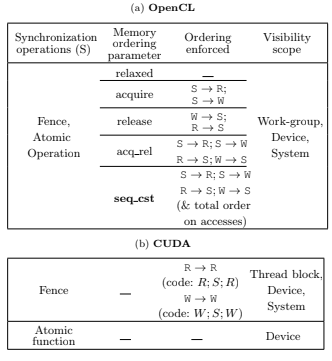
\includegraphics[width=0.7\textwidth]{figures/cudagpu}
  \caption{Programorder von OpenCL und CUDA \cite{eesmog}.}
  \label{Fig:cudagpu}
\end{figure}

Abbildung 12 zeigt in der ersten Spalte die Synchronisationsoperationen, die OpenCL und CUDA zur Verfügung stellen.
Beide arbeiten mit Fences, die auch Barrieren genannt werden \cite{fences}. 
Nur innerhalb zweier Fences dürfen Speicheroperationen synchronisiert werden \cite{smcmtutorial}. 
OpenCL verfügt über vier verschiedene Programorders, die sich in aquire, release, acq\_rel und seq\_cst unterteilen.
Man kann an dieser Stelle bereits Parallelen zu RC erkennen.
Eine neue Regel die auffällt ist seq\_cst.  Diese stellt sicher, dass Speicheroperationen, die nach einer Synchronisation anfangen, 
nicht vor dieser Synchronisation enden und umgekehrt. Dies führt zwar zu einer Überlappung der Operationen, aber verhindert eine Speicherverletzung \cite{eesmog}.

CUDA stattdessen kennt nur zwei Programorders: R → R und W → W.
Dabei ist zu beachten, dass R und W jeweils auch Synchronisationsoperationen darstellen können.
Dieses Modell kommt mit weniger Funktionen aus, da es auf eine weitläufige Speicheraufteilung verzichtet \cite{eesmog}.

Ein weiteres Feature, das beide GPUPUs gemeinsam haben, sind die Visibility Scopes.
Wird eine Synchronisation getriggert, geschieht das immer im Zusammenhang mit festgelegten Scopes, die 
auch als hierarchische Reichweite bezeichnet werden können.

Man unterscheidet zwischen System, Device und work-group (OpenCL)/thread-block (CUDA).

Wird eine Synchronisation also systemweit angewandt, so sind sowohl GPU, CPU, als auch etwaige andere Rechenunits, wie z.B. eine zweite GPU davon betroffen.
Das Scope Device beschäftigt sich nur mit der GPU, auf dem die Synchronisation getriggert wurde, selbst, während das dritte Scope 
nur einzelne Threadcluster synchronisiert \cite{denovor}.








\section{Zusammenfassung und Fazit}
Wenn man sich vor Augen hält, wie sich die Applikationsentwicklung für GPUs im Bezug auf Speicherkonsistenz entwickelt hat,
fällt auf, dass dank neuerer Konzepte wie OpenCL und CUDA eine bequeme Möglichkeit geschaffen wurde.
Zwar bilden das Weak Consistency Model und das Release Consistency Model ein solides Grundgerüst für eine performantere datenparallele Entwicklung \cite{mcm5} - im Gegensatz zum reinen sequentiellen Konsistenzmodell - allerdings sind sie für CPUs entworfen worden und das spiegelt sich in vielen vorgestellten Problematiken wieder:
Durch den hierarchischen Speicheraufbau und die schiere Anzahl an Threads einer GPU müssen neue Techniken entworfen werden, die die CPU-Modelle jedoch zumindest als Vorbild nutzen können.

Vor allem OpenCL hat sich dank der platformübergreifenden Eigenschaft und der umfangreichen Funktionalität auf dem Markt etabliert.
Es bietet sowohl mehr Formalität und Flexibilität, als einfachere Möglichkeiten, Speicheroperationen zu handhaben als CUDA.
Die von Nvidia entwickelten Fences reichen im Vergleich zu den unterschiedlichen Synchronisationsalternativen bei OpenCL nicht aus,
um kritische Operationen ausreichend zu schützen \cite{gpucc}. 
Bei OpenCL ist dies einfacher, aber auch hier muss der Programmierer genau darauf achten, die richtigen Operationen anzusetzen.

Wer heute einen Grafikchip entwickeln möchte oder auf einem solchen programmieren, der fährt am besten mit OpenCL und den zugrundeliegenden schwachen Konsistenzmodellen.

Noch werden die Dokumentation und auch die Informationen, die von den GPU-Herstellern kommen, spärlich gehandhabt.
 Trotzdem entdecken immer mehr Forscher Entwickler die hervorragenden datenparallelen Eigenschaften von GPUs für sich, weshalb es nur noch eine Frage der Zeit sein kann, bis sich neue, auf schwachen Konsistenzmodellen basierende, Architekturen etablieren.  



\newpage



\nocite{*}

\printbibliography


\end{document}
